\subsection{Arduino}

\par
Arduino es una plataforma de electrónica de código abierto basada en hardware y software fácil de usar. Las placas Arduino pueden leer entradas (luz en un sensor, un dedo en un botón o un mensaje de Twitter) y convertirlo en una salida, activar un motor, encender un LED y publicar algo en línea. Puede decirle a su placa qué hacer enviando un conjunto de instrucciones al microcontrolador en la placa. Para hacerlo, utiliza el lenguaje de programación Arduino (basado en \textquotedblleft Wiring\textquotedblright) y el software Arduino (IDE), basado en \textquotedblleft Processing \textquotedblright\cite{arduino-intro}.

\begin{figure}[H]
	\centering
	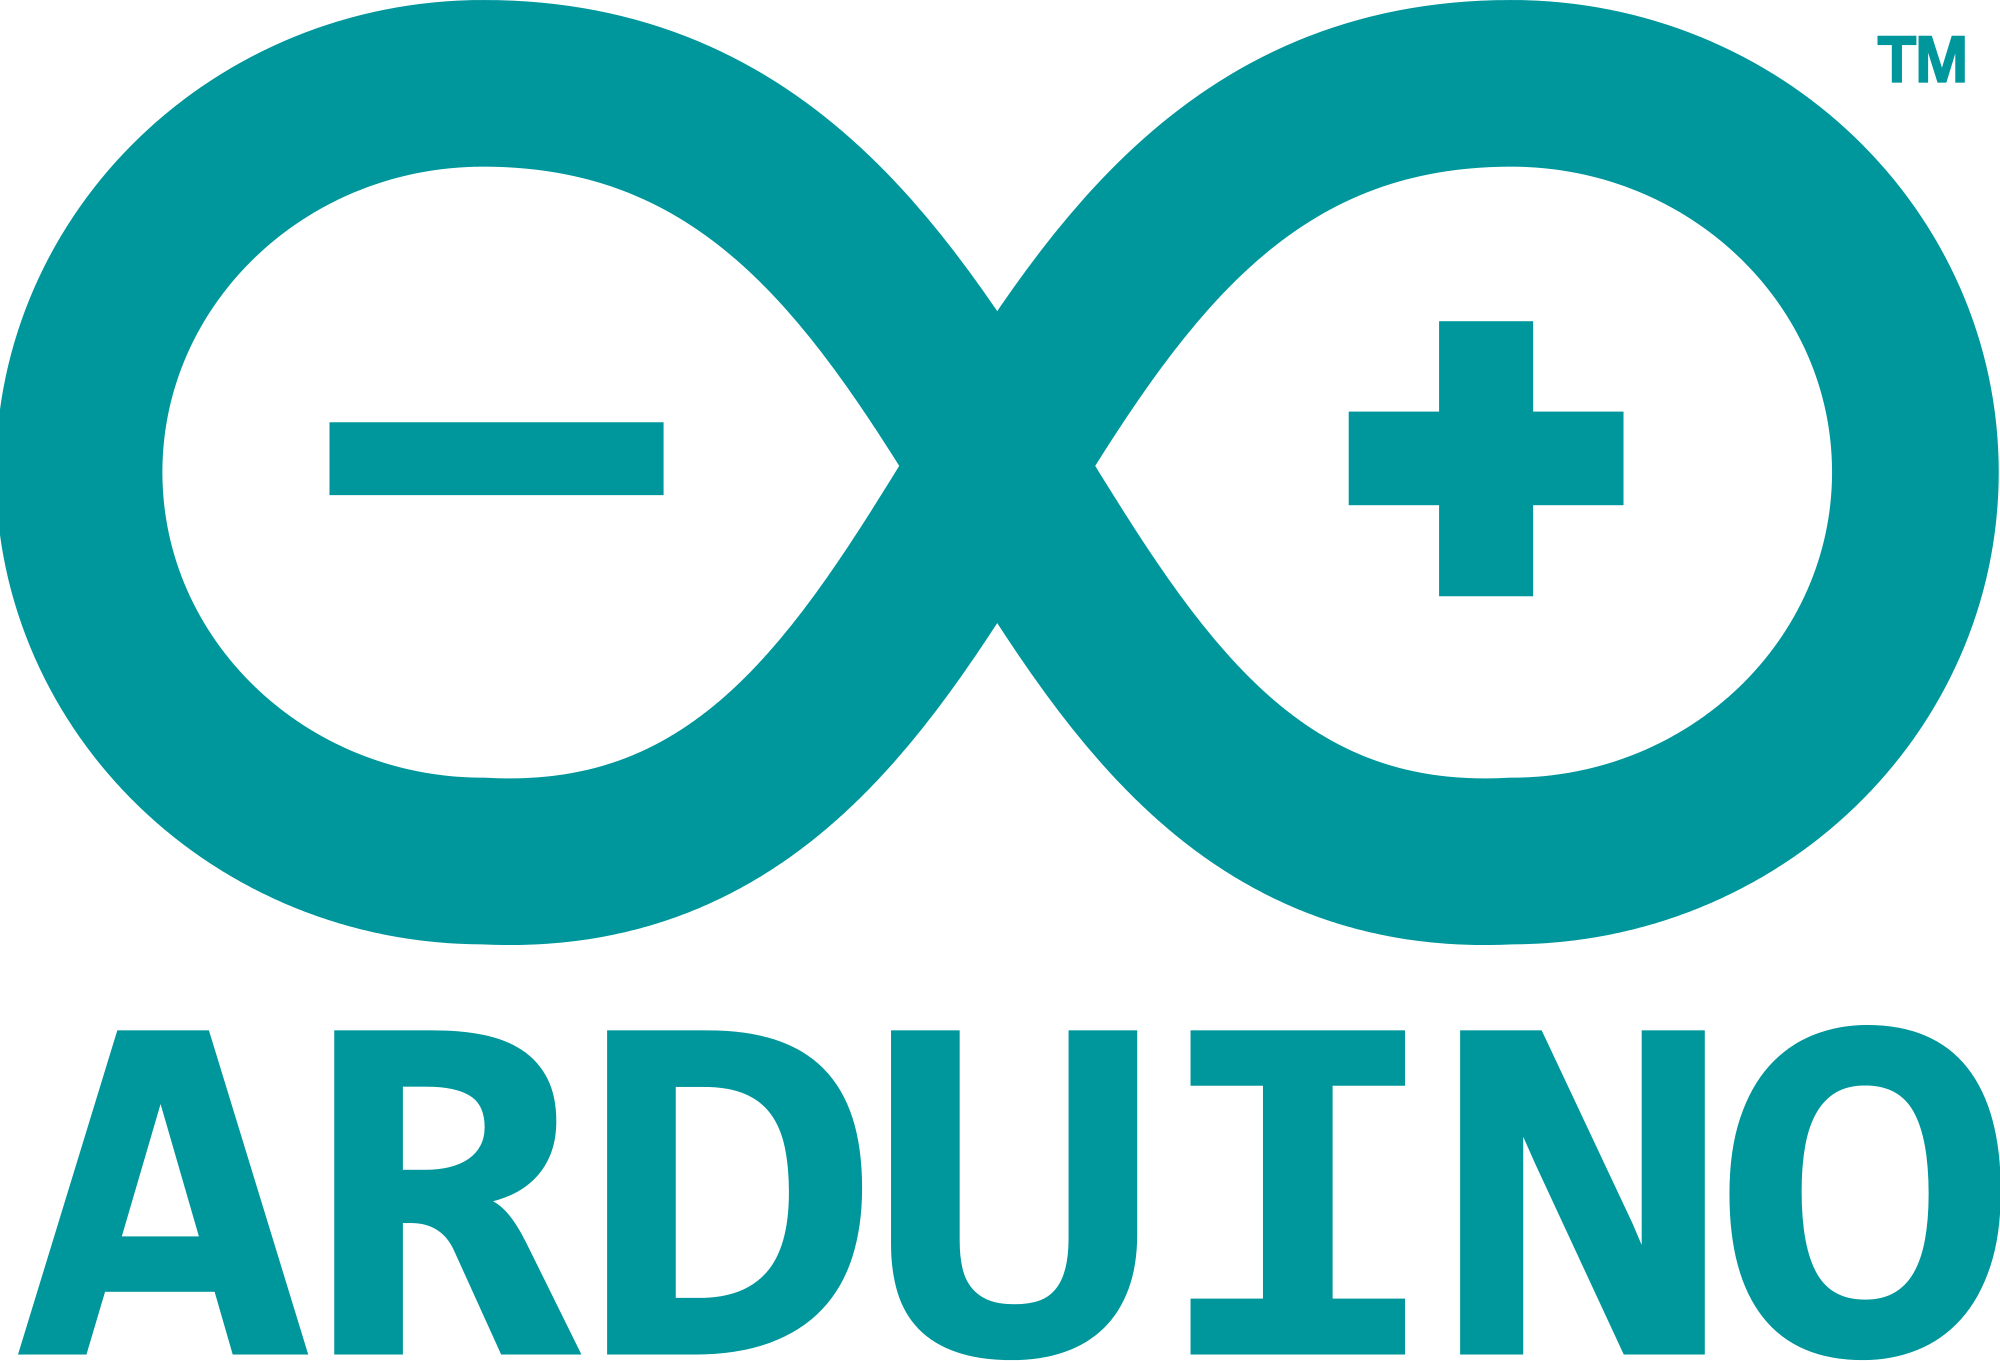
\includegraphics[width=5cm, height=4cm]{arduino1.png}
	\caption{Logo Oficial de Arduino}
\end{figure}

\par \noindent
Con los años, Arduino ha sido el cerebro de miles de proyectos, desde objetos cotidianos hasta complejos instrumentos científicos. Una comunidad mundial de fabricantes (estudiantes, aficionados, artistas, programadores y profesionales) se ha reunido en torno a esta plataforma de código abierto, sus contribuciones se han añadido a una increíble cantidad de conocimiento accesible que puede ser de gran ayuda para principiantes y expertos por igual\cite{arduino-intro}.

\begin{figure}[H]
	\centering
	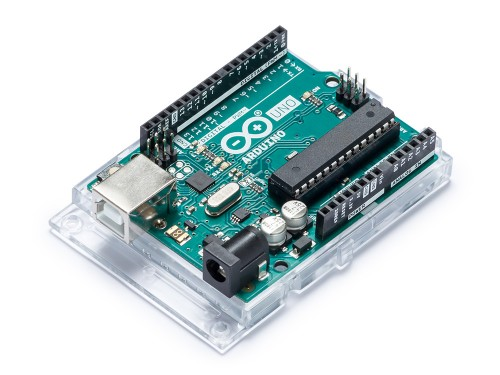
\includegraphics[width=6cm, height=5cm]{arduino2.jpg}
	\caption{Placa Arduino Uno}
\end{figure}

\par \noindent
Arduino nació en el Ivrea Interaction Design Institute como una herramienta fácil para el prototipado rápido, dirigido a estudiantes sin experiencia en electrónica y programación. Tan pronto como llegó a una comunidad más amplia, la placa Arduino comenzó a cambiar para adaptarse a las nuevas necesidades y desafíos, diferenciando su oferta de simples placas de 8 bits para productos para aplicaciones IoT, wearable, impresión 3D y entornos integrados. Todos los tableros Arduino son completamente de código abierto, lo que permite a los usuarios construirlos de forma independiente y eventualmente adaptarlos a sus necesidades particulares. El software también es de código abierto y está creciendo a través de las contribuciones de los usuarios en todo el mundo\cite{arduino-intro}.

\begin{figure}[H]
	\centering
	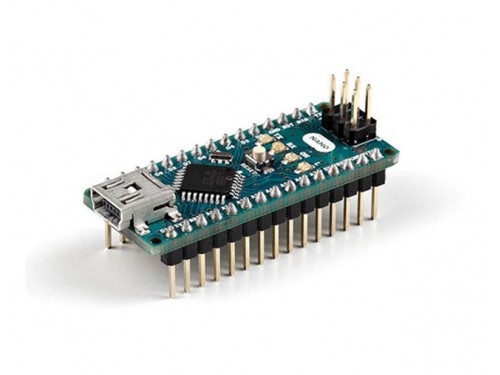
\includegraphics[width=6cm, height=5cm]{arduino3.jpg}
	\caption{Placa Arduino Nano}
\end{figure}

\subsubsection{Módulos Arduino}

\par
Los módulos de Arduino son esencialmente placas de circuitos independientes que integran uno o múltiples circuitos integrados, sensores, pantallas LCD, componentes electrónicos y una interfaz de pines para una comunicación sencilla con la placa Arduino. Los módulos nos permiten agregar funcionalidad a nuestra placa arduino y son como piezas de un rompecabezas donde el resultado final es el prototipo deseado.

\par \noindent
Los componentes electrónicos principales son los siguientes:

\paragraph{Resistencia}
Son usados para establecer corrientes de operación y niveles de señal. Resistencias se utilizan en los circuitos de alimentación para reducir los voltajes al disipar la potencia, medir las corrientes y descargar los capacitores después de que se desconecta la energía. Una resistencia está hecha de elementos conductores (carbono, o una película delgada de metal o carbono, o un cable de baja conductividad), con un cable o contactos en cada extremo\cite{artofelectronics}. Se caracteriza por su resistencia y es definido por:

$$R = V/I$$

\begin{nscenter}
	Ley de Ohm: Donde R es de Resistencia, V de Voltaje e I de corriente.
\end{nscenter}

\begin{figure}[H]
	\centering
	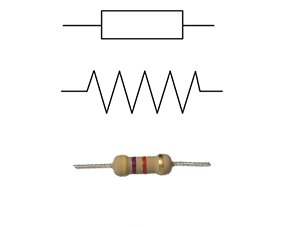
\includegraphics[width=8cm, height=6cm]{resistor1.png}
	\caption{Ejemplo de Resistor y Simbología}
\end{figure}

\paragraph{Capacitor }
Un capacitor (el nombre antiguo era
condensador) es un dispositivo que tiene dos cables que sobresalen y tiene la propiedad\cite{artofelectronics} :
$$Q = CV$$ 

\begin{nscenter}
	Donde Q es carga almacenada en coulombs, C la capacitancia en faradios y V es el diferencia de potencia en voltios.
\end{nscenter}

\begin{figure}[H]
	\centering
	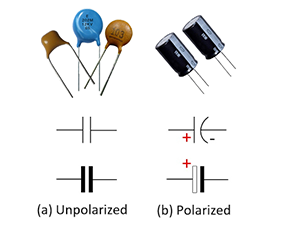
\includegraphics[width=8cm, height=6cm]{capacitor1.png}
	\caption{Ejemplo de Capacitor y Simbología}
\end{figure}

\par \noindent
Los capacitores esencialmente almacenan energía, pero es principalmente utilizado en corriente directa para filtrar picos de voltage provenientes de la fuente de la fuente de poder\cite{artofelectronics}.

\paragraph{Inductor}
Están estrechamente relacionados con condensadores: la tasa de cambio de corriente en un inductor es proporcional al voltaje aplicado a través de él (para un condensador es al revés, la tasa de cambio de voltaje es proporcional a la corriente a través de él) \cite{artofelectronics}. La ecuación de definición para un inductor es:
$$V = L\frac{dl}{dt}$$

\par \noindent
donde $L$ se llama inductancia y se mide en henrios
(o $mH$, $pH$, $nH$, etc.). Poniendo un voltaje constante a través de un
inductor hace que la corriente se eleve como una rampa (en comparación con un condensador, en el que una corriente constante causa el voltaje subir como una rampa); l $V$ a través de 1 $H$ produce una corriente que aumenta a 1 amperio por segundo \cite{artofelectronics}.

\begin{figure}[H]
	\centering
	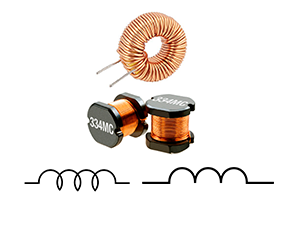
\includegraphics[width=8cm, height=6cm]{inductor1.png}
	\caption{Ejemplo de Inductor y Simbología}
\end{figure}

\par \noindent
Al igual que con los capacitores, la energía invertida en el aumento de la corriente en un inductor se almacena internamente, aquí en la forma de campos magnéticos \cite{artofelectronics}.

\par \noindent
Ya definidos los componentes electricos que componen los modulos de arduino procedemos a explicar los dos modulos utilizados en este proyecto \cite{artofelectronics}.

\clearpage

\paragraph{Modulo Bluetooth HC-05}
El módulo HC-05 es un módulo Bluetooth SPP (Serial Port Protocol por sus siglas en ingles) fácil de usar, diseñado para la configuración de conexión en serie inalámbrica transparente. El módulo Bluetooth HC-05 se puede utilizar en una configuración maestra o esclava, lo que la convierte en una excelente solución para la comunicación inalámbrica .Este puerto en serie del módulo bluetooth es completamente calificado Bluetooth V2.0 + EDR (Enhanced Data Rate) Modulación de 3Mbps con un completo transceptor de radio de 2.4GHz y banda de base\cite{bluetooth}.

\begin{figure}[H]
	\centering
	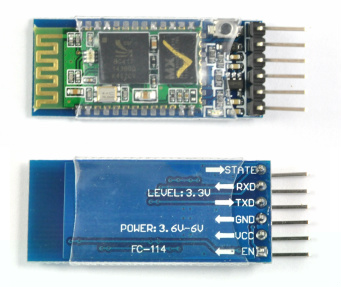
\includegraphics[width=8cm, height=6cm]{modulos1.jpg}
	\caption{Placa HC-05 Modelo ZS-040}
\end{figure}

\paragraph{Modulo Wi-Fi nRF24L01+}
El nRF24L01+ es un transceptor de 2.4GHz de un solo chip con un motor de protocolo de banda base integrado
, adecuado para aplicaciones inalámbricas de muy baja potencia. El nRF24L01 + está diseñado
para el funcionamiento en la banda de frecuencia ISM mundial a 2.400 - 2.4835GHz\cite{nrf}.

\par \noindent
Para diseñar un sistema de radio con nRF24L01 +, simplemente necesita una MCU (microcontrolador) y algunos componentes externos pasivos.

\par \noindent
El motor de protocolo de banda base integrado se basa en la comunicación por paquetes
y es compatible con varios modos, desde la operación manual hasta la operación de protocolo autónomo avanzado. 
Los FIFOs internos aseguran un flujo de datos sin problemas entre la interfaz de radio y la MCU del sistema. El motor mejorado reduce el costo del sistema mediante el manejo de todas las operaciones de capa de enlace de alta velocidad\cite{nrf}.

\begin{figure}[H]
	\centering
	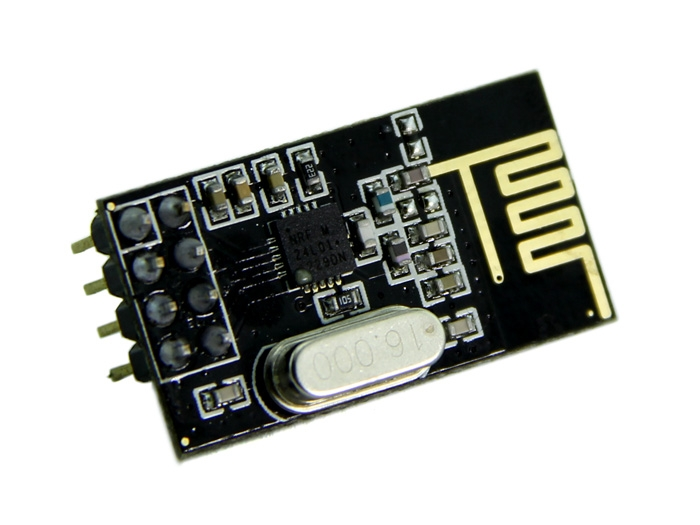
\includegraphics[width=8cm, height=6cm]{modulos2.jpg}
	\caption{Placa nRF24L01+}
\end{figure}

\par \noindent
El modulo nRF24L01+ admite una velocidad de datos de aire de 250 kbps, 1 Mbps y 2 Mbps.
La alta velocidad de datos de aire combinada con dos modos de ahorro de energía hacen que el nRF24L01+ sea muy adecuado para ultra bajo
diseños de energía\cite{nrf}.

\par \noindent
Los modulos previamente mencionados son elementos indispensables para enviar y recibir información entre nuestro prototipo y la aplicación móvil. El prototipo debe ser capaz de capturar mediciones de temperatura de manera precisa; por ende se requiere un sensor eficaz y eficiente.

